\secnumbersection{DEFINICIÓN DEL PROBLEMA} 

%Se debe definir el problema, es importante no confundir definir el problema con describir la solución. Por ejemplo: ``diseñar una arquitectura e implementar una plataforma ...'' es una solución, no un problema.

%Algunos elementos que podrían ir en este capítulo son (no es necesario que vayan todos):
%\begin{itemize}
 %   \item Breve descripción del contexto donde se realizará la memoria (organización, línea dentro de la Informática en la que se basa, etc.)
 %   \item ¿Qué y cómo se realiza actualmente la situación que mejorarás con tu memoria?
  %  \item ¿Qué actores o usuarios están involucrados?
  %  \item ¿Qué dificultades tienen esos actores actualmente? ¿cuántos son? (ideal si se pueden poner estadísticas para así saber si existe un mercado razonable para la solución que propondrás en tu memoria, en el fondo saber cuántas personas u organizaciones tienen el mismo problema que estás definiendo)
   % \item ¿Qué podría pasar si en el corto o mediano plazo no se solucionan esas dificultades (¿es decir, si no se hiciera tu memoria, qué pasaría?; en el fondo justificar por qué conviene hacer tu memoria, ¿cuál es la motivación o interés de hacerla?).
   % \item ¿Qué competencia existe actualmente? (a lo mejor ya existe una solución al problema, pero por qué no sirve, o por qué tu solución sería mejor, también se puede enfocar a si este problema existe en otras realidades y cómo ha sido solucionado allí).
%    \item Precisar los objetivos y alcances de la memoria (o solución al problema).
%\end{itemize}

%En este capítulo, de ser necesario puede usar referencias bibliográficas (velar porque sean recientes), una cita de ejemplo \cite{schwab2002cure} y otras más \cite{georget1994study,beaumont1990patient}.

%Recuerde poner notas al pie de página que sean explicativas \footnote{Este es un ejemplo de una nota al pie de página. Puede indicar alguna URL, definiciones, aclarar alguna información pertinente del texto, citar algunas referencias, etc..}.

\subsection{Contexto}

Los estudios en la física de partículas buscan responder la pregunta "¿De qué se compone la materia?". Esto ha llevado a la búsqueda del componente principal de la materia\footnote{El componente más pequeño e indivisible}. Hasta hace algunos años las partículas subatómicas; electrón, neutrón y protón, eran conocidas como las partículas fundamentales\footnote{Partículas sin sub-estructura conocida.} de la materia. Sin embargo, en trabajos más recientes se ha demostrado que los neutrones y protones sí poseen una sub-estructura compleja \cite{Griffiths}, y al mismo tiempo se han descubierto decenas de partículas más \cite{PhysRevD.98.030001}. Algunas partículas fundamentales (o elementales) se pueden observar en la Figura \ref{fig:partics}.

\begin{figure}[h]
  \centering
  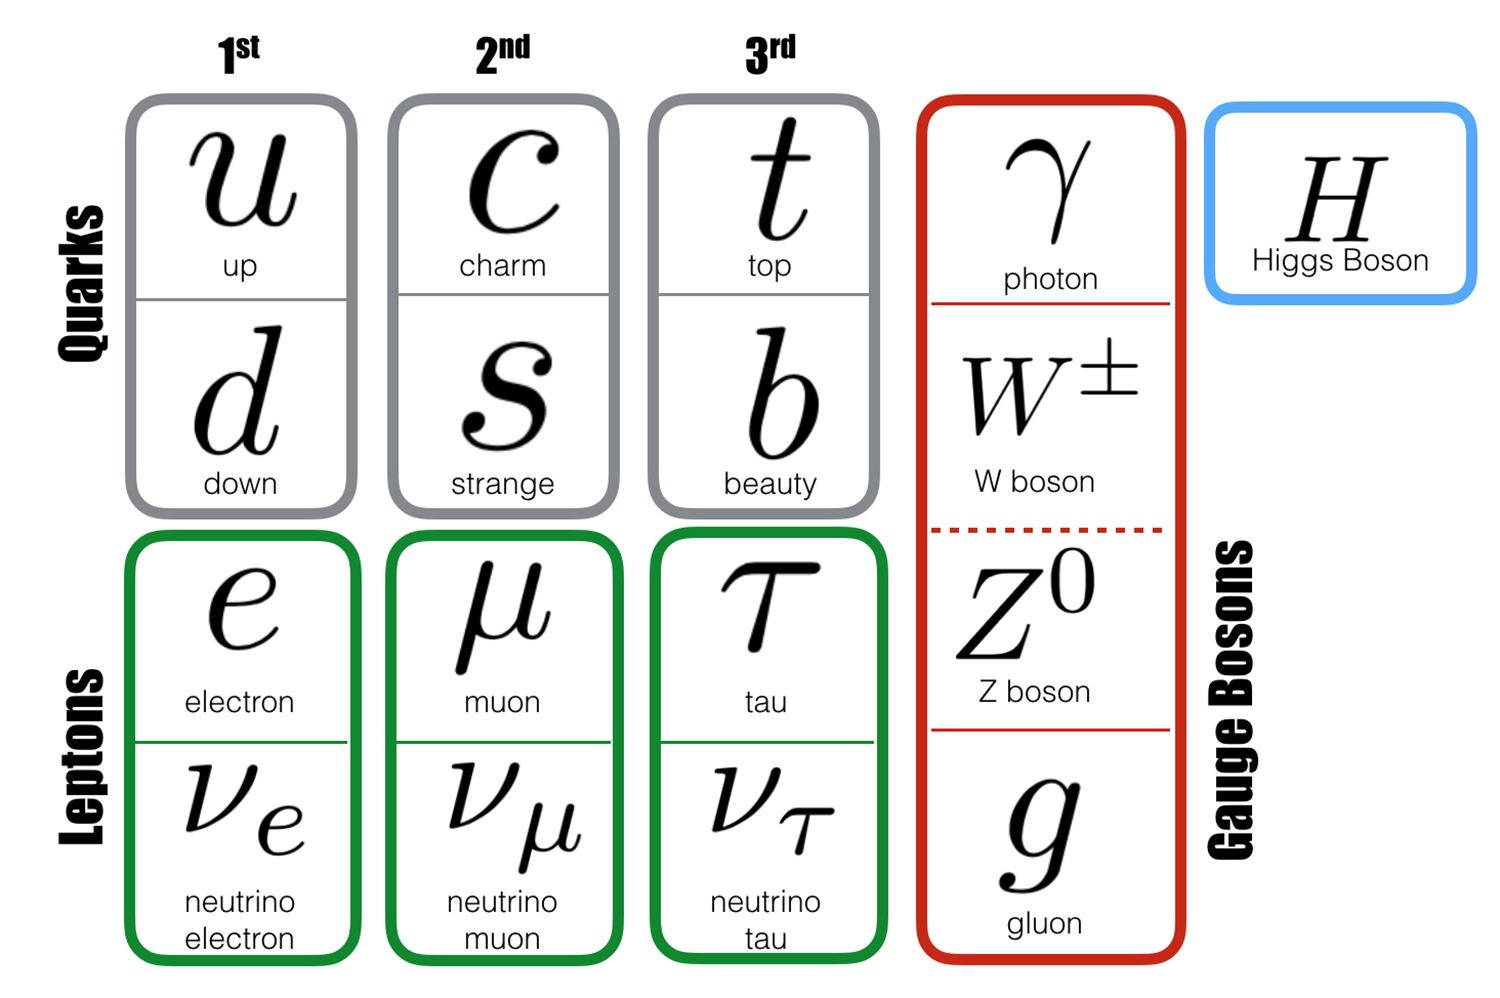
\includegraphics[width=10cm]{figures/image10.png}
  \caption[Diagrama del modelo estándar.]{Partículas elementales del modelo estándar, divididas por tipo: gris (quarks), azul (bosón de Higgs), rojo (bosones de Gauge) y verde (leptones), y por familias: primera, segunda y tercera, en columnas respectivas.
  \source{\url{https://www.physik.uzh.ch/en/researcharea/lhcb/outreach/StandardModel.html}}}
  \label{fig:partics}
\end{figure}

\subsubsection{Modelo Estándar}
El modelo estándar de la física de partículas es la teoría matemática que describe la interacción fuerte, débil, electromagnética y gravitacional entre leptones y quarks, a través de campos producidos por ellos mismos \cite{Cottingham}. Además, el modelo estándar presenta los procesos a los que se pueden someter las partículas y las diferentes combinaciones de estos permiten la conformación de sistemas de procesos más complejos, los cuales pueden ser comparados con observaciones experimentales. Un proceso de ejemplo se puede observar en el diagrama de la Figura \ref{fig:feynman1}.

\begin{figure}[]
    \centering
    \feynmandiagram [horizontal=a to b] {
        i1 [particle=\(e^{-}\)] -- [fermion] a -- [fermion] i2 [particle=\(e^{+}\)],
  a -- [photon, edge label=\(\gamma\)] b,
  f1 [particle=\(\mu^{+}\)] -- [fermion] b -- [fermion] f2 [particle=\(\mu^{-}\)],
    };
    \caption[Diagrama de Feynman para la producción del par $\mu^+\mu^-$.]{Diagrama de Feynman para la producción del par $\mu^+\mu^-$ en colisiones $e^+ e^-$.
    \source{Elaboración propia.}}
    \label{fig:feynman1}
\end{figure}

\subsubsection{Large Hadron Collider (LHC)}
Pese a que el modelo estándar describe los fenómenos del campo de la física de partículas, este aún está incompleto. Por ello, experimentos como el \emph{Large Hadron Collider} (\acrshort{lhc}) del CERN, se dedican a realizar experimentos con el objetivo de generar nuevo conocimiento que se sume al modelo estándar.
%
El \acrshort{lhc} es catalogado como el acelerador\footnote{Producen rayos de partículas cargadas, las cuales son aceleradas mediante el aumento de los campos electro-magnéticos.} 
%
y colisionador\footnote{Tipo de acelerador de partículas utilizado para producir choques entre dos rayos de partículas.} 
%
de hadrones\footnote{Partículas formadas por dos o más quarks.} 
%
más avanzado a nivel mundial, y está ubicado en Ginebra, Suiza.
%
Su objetivo principal es la investigación de la validez y restricciones del modelo estándar. 
%
EL LHC es una acelerador subterráneo circular de 27 km de circunferencia.
%
Dentro del LHC, haces de protones colisionan a una frecuencia de 40 MHz, y a altísimos niveles de energías del orden de los 13 TeV.
%
En la Figura \ref{fig:lhc} se puede observar un diagrama del \acrshort{lhc} y la ubicación de los experimentos en su anillo.

\begin{figure}[h]
  \centering
  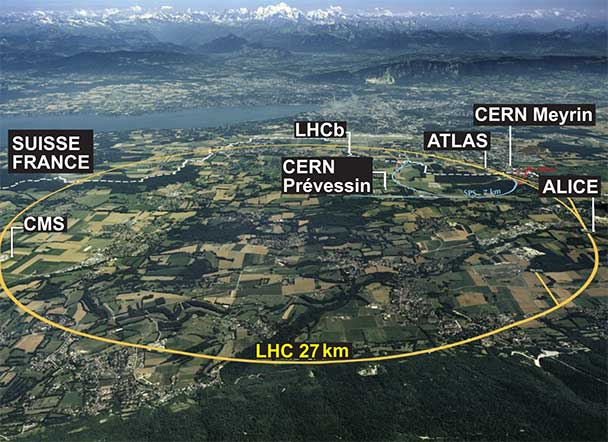
\includegraphics[width=12cm]{figures/image1.jpg}
  \caption[Esquema del LHC.]{Esquema del \acrshort{lhc} en \acrshort{cern}.
  \source{\url{https://www.aps.org/publications/apsnews/201409/backpage.cfm}}}
  \label{fig:lhc}
\end{figure}

\subsubsection{Experimento ATLAS}
Existen siete experimentos en el \acrshort{lhc} \cite{ExpWP}: \acrshort{atlas}, \acrshort{cms}, ALICE, \acrshort{lhcb}, TOTEM, LHCf y MoEDAL, los cuales utilizan detectores para estudiar las partículas producidas por las colisiones en el acelerador. 
%
\acrshort{atlas} ({\bf A} {\bf T}oroidal {\bf L}HC {\bf A}pparatuS) es uno de los experimentos más grandes del LHC, y su detector tiene 44 metros de largo, 25 metros de diámetro y pesa alrededor de 7000 toneladas \cite{ATLASWP}. 
%
ATLAS  está diseñado para detectar partículas producidas en colisiones, o {\bf eventos}, gracias a millones de sensores que están especialmente diseñados para medir las propiedades de tales partículas, como su momentum, energía y carga eléctrica. 
%
ATLAS puede distinguir entre fotones, electrones, muones y ``jets'' de partículas hadrónicas iniciados por quarks, además de determinar el vértice donde ocurrió la colisión de interés, así como también las muchas otras interacciones que ocurren en cada evento.  


ATLAS puede detectar más de un billón de colisiones por segundo, lo cual produce alrededor de 60 millones de megabytes por segundo. 
%
Debido a la gran cantidad de colisiones o eventos producidos en el LHC, no es posible almacenar los gigantes volúmenes de datos generados, por lo tanto, se realiza una selección de eventos utilizando un sistema especializado, denominado \emph{trigger} (o disparador) \cite{Armstrong2004}. 
%
Este sistema registra sólo los eventos que son interesantes desde el punto de vista de la física de partículas de altas energías. 
%
En particular, el experimento ATLAS extrae aproximadamente 1 de cada 100.000 eventos generados por el LHC, lo que significa almacenar más de $20 \text{ Pb}$ de datos por año \cite{Radovic2018}. 


\begin{figure}[]
  \centering
  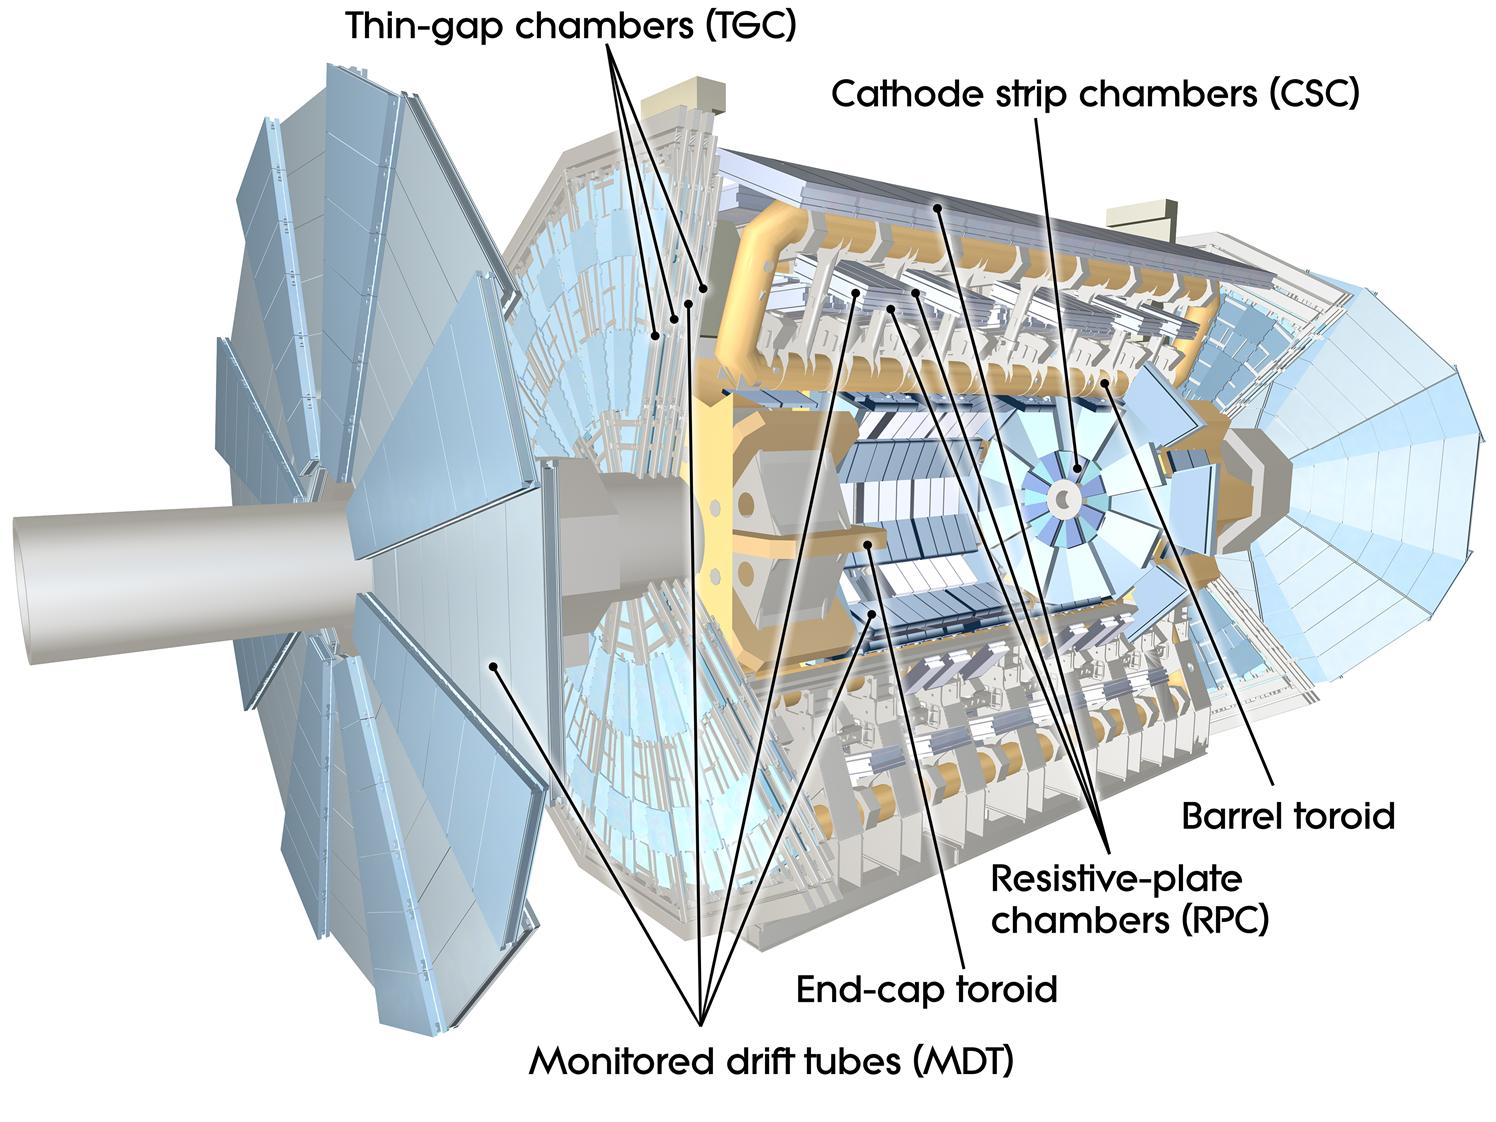
\includegraphics[width=9cm]{figures/image2.jpg}
  \caption[Esquema del experimento ATLAS.]{Esquema del experimento \acrshort{atlas} que revela parte interna del detector.
  \source{\url{https://cds.cern.ch/record/1095929}}} \label{fig:atlasdet}
\end{figure}

\subsubsection{Clasificación de Eventos}
La  identificación o clasificación de los eventos producidos en el LHC, es una de las tareas más importantes que desarrolla la comunidad científica del CERN.
%
La clasificación de estos eventos es fundamental para mejorar la precisión de los resultados actuales, y también para buscar nuevos fenómenos en el campo de la física de altas energías.
%

La clasificación de eventos ---o la separación de los eventos tipo {\bf señal} de los eventos tipo {\bf background}--  
es un desafío debido a que la señal es muy poco frecuente en comparación al background.
%desde un {\bf background} dominante.
%
Por ejemplo, un bosón de Higgs se produce  aproximadamente una vez cada mil millones de colisiones protón-protón generadas en el LHC.

%Volviendo a las partículas elementales, el bosón de Higgs es una partícula cuya existencia fue predicha hace más de 50 años \cite{Higgs1964}. Su importancia yace en que es el última pieza del modelo estándar, y sin la corroboración de su existencia, los principios fundamentales planteados por el modelo estándar, colapsarían.

Si bien, los experimentos \acrshort{atlas} \cite{Aad2012,ATLASweb} y \acrshort{cms} \cite{Chatrchyan2012} del \acrshort{lhc}, anunciaron el descubrimiento del bosón de Higgs en el año 2012, los investigadores del \acrshort{lhc} siguen enfocados en mejorar los niveles de precisión de los resultados ya obtenidos, y continúan con la búsqueda de indicios de \textit{nueva física} que vaya más allá del modelo estándar.
%
%
%
\subsection{Descripción del Problema}
%
Como ya hemos mencionado, el análisis de datos en Física de Partículas incluye como tarea principal la identificación de eventos de interés. 
%
Esto se lleva a cabo a través de un proceso de \textit{clasificación} o selección, en el que se identifican los datos correspondientes al evento buscado (señal), por sobre el resto de los datos o \textit{background} \cite{BiniClass}. 
%
Así, los conceptos evento, señal y background  se entenderán como:
%
\begin{itemize}
    \item \emph{{\bf Evento:} Momento posterior a la ocurrencia de una interacción fundamental entre partículas subatómicas. Por ejemplo, una colisión entre dos partículas \cite{symmWP}.}
    
    \item \emph{{\bf Señal:} Evento de interés desde el punto de vista físico. En este trabajo la señal que se analizará corresponde a la producción de un par de bosones de Higgs (o di-Higgs).} 
    
    \item \emph{{\bf Background:} Cualquier otro evento diferente al de la señal.}
    
\end{itemize}

%
\textbf{Así, en este trabajo el problema a abordar corresponde a la clasificación de eventos detectados por el experimento ATLAS, para identificar la producción de un par de bosones de Higgs (o di-Higgs).}

\subsubsection{El Bosón de Higgs}

Un \textit{bosón de Higgs} se produce a partir de los subproductos de una colisión de dos rayos de partículas que fueron acelerados y chocan a muy altas energías, dentro de un detector como el \acrshort{lhc}.
%
Algunas de estas producciones pueden ser representadas por los diagramas de Feynman de la Figura \ref{fig:pchan}. 
%
El bosón de Higgs se produce durante un tiempo muy breve, con una vida media de $1.56 \times 10^{-22}$ segundos \cite{Mellado2012}. 
%
Debido a que el bosón de Higgs decae\footnote{Proceso espontáneo en el que una partícula inestable se transforma en otras partículas.} muy rápido, los detectores de partículas no pueden detectarlo directamente, sino que lo identifican a partir de un proceso de \textit{reconstrucción} \cite{Giardino2012}, lo cual consiste en reproducir el decaimiento de las partículas partiendo por los productos finales de la colisión, hasta la colisión de origen. 
%
La idea es buscar aquellos canales de decaimiento\footnote{Posibles transformaciones de una partícula al decaer.} que coincidan con los del bosón de Higgs. 
%
Estos últimos son presentados en la Tabla \ref{tab:decays}.

\begin{figure}[h]
  \centering
  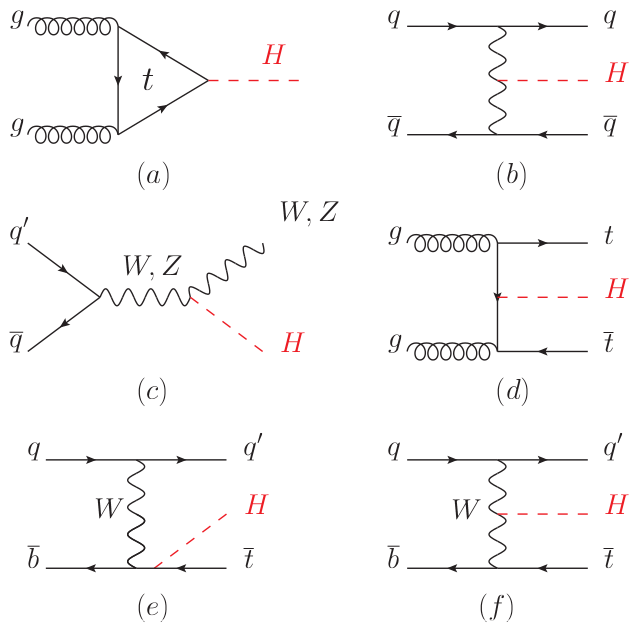
\includegraphics[width=10cm]{figures/image8.png}
  \caption[Diagramas de Feynman para la producción del bosón de Higgs.]{Diagramas de Feynman para la producción del bosón de Higgs a partir de diferentes partículas: \emph{(a)} Fusión de gluones \cite{glover1988higgs}, \emph{(b)} fusión vector-bosón \cite{Dicus1985}, \emph{(c)} irradiación de Higgs (o producción asociada al bosón de Gauge) \cite{Brein2013vh}, \emph{(d)} producción asociada al par de quarks top \cite{kunszt1984associated} o al par de quarks bottom \cite{khachatryan2015search}, \emph{(e-f)} producción asociada a un quark top \cite{maltoni2001associated}.
  \source{\cite{PhysRevD.98.030001}}}
  \label{fig:pchan}
\end{figure}

\begin{table}[h]
\centering
\begin{tabular}{c|c|c|c|c|c|c|c|}
\cline{2-8}
 & \multicolumn{7}{c|}{Canales de decaimiento} \\ \hline
\multicolumn{1}{|l|}{$H \rightarrow$} & $\gamma\gamma$ & $ZZ$ & $W^+ W^-$ & $\tau^+ \tau^-$ & $b\bar{b}$ & $Z\gamma$ & $\mu^+ \mu^-$ \\ \hline
\end{tabular}
\caption[Resumen de los \textit{canales de decaimiento} del bosón de Higgs.]{Resumen de los \textit{canales de decaimiento} del bosón de Higgs. 
\source{Elaboración propia.}}
\label{tab:decays}
\end{table}

El rango de energías con las que se puede producir un bosón de Higgs, va desde 115 a 190 GeV aproximadamente \cite{al2006}. Sin embargo, con energías menores a 150 GeV se produce mucho background, lo cual dificulta la detección de la partícula. Además, la probabilidad de producir un bosón de Higgs en cualquier colisión, es muy baja. En el \acrshort{lhc} se espera la producción de sólo un bosón de Higgs por cada diez billones de colisiones \cite{Baglio2011}.

\subsubsection{Producción de di-Higgs}

La producción del par de bosones de Higgs (di-Higgs) es un evento aún más raro que la producción de un sólo Higgs, con una taza de producción aproximadamente mil veces más pequeña que la generación de un solo bosón de Higgs \cite{doublehWP}.
%
En el modelo estándar, las producciones del par de Higgs proceden de un ciclo\footnote{Diagrama de Feynman conectado.} ---principalmente de top quarks---, o del autoacoplamiento trilineal\footnote{El \textit{autoacoplamiento triple del bosón de Higgs} se refiere a la interacción entre tres bosones de Higgs, donde un Higgs decae en dos Higgs de menor energía.} de un bosón de Higgs \cite{DiVita2017}, estos pueden ser representados por los diagramas de Feynman, \emph{(a)} y \emph{(b)} respectivamente, de la Figura \ref{fig:pchan2}. 
%
Los estados finales más prometedores\footnote{Presentan mayor sensibilidad para detectar el decaimiento del di-Higgs.} en decaimientos de un par de bosones de Higgs ($hh$) se muestran en la Tabla \ref{tab:decays2}.
%
%
\begin{figure}[h]
  \centering
  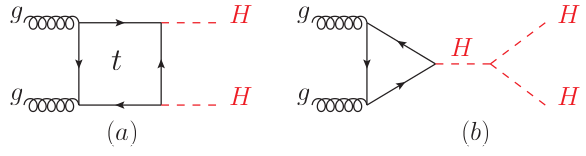
\includegraphics[width=10cm]{figures/image9.png}
  \caption[Diagramas de Feynman para la producción del par de bosones Higgs.]{Diagramas de Feynman para la producción del par de bosones Higgs a partir de: \emph{(a)} ciclo de quark top y quark b, y \emph{(b)} auto-acoplamiento del bosón de Higgs.
  \source{\cite{PhysRevD.98.030001}}}
  \label{fig:pchan2}
\end{figure}

\begin{table}[h]
\centering
\begin{tabular}{c|c|c|c|c|c|}
\cline{2-6}
 & \multicolumn{5}{c|}{Canales de decaimiento} \\ \hline
\multicolumn{1}{|l|}{$hh \rightarrow$} & $b\bar{b}\gamma\gamma$ & $b\bar{b}\tau\tau$ & $b\bar{b}WW$ & $b\bar{b}b\bar{b}$ & $WWWW$ \\ \hline
\end{tabular}
\caption[Resumen de los \textit{canales de decaimiento} del par de bosones de Higgs.]{Resumen de los \textit{canales de decaimiento} del par de bosones de Higgs. 
\source{Elaboración propia.}}
\label{tab:decays2}
\end{table}

Uno de los objetivos del \acrshort{cern} con respecto al \acrshort{lhc}, es alcanzar el nivel de energía de los 100 TeV \cite{Arkani2016}, produciendo colisiones mucho más masivas que las que se han producido hasta ahora. Como consecuencia, el número de datos se duplicará, lo cual permitirá generar mayor cantidad de material de estudio para el análisis de diferentes eventos como la producción del par de bosones de Higgs.

\subsection{Solución actual}

Los métodos más utilizados para resolver este problema hasta el día de hoy, se basan en \textit{técnicas de subestructura de jets}\footnote{Un jet es un \emph{chorro} de \textit{hadrones}, representada en los diagramas por un cono, como resultado de la colisión altamente energética entre dos partículas.} (o \textit{algoritmos de jet}\footnote{Algoritmos que reducen la información de una colisión, con lo que se reconstruyen y definen los jets posteriormente.}) \cite{Chekanov2003}, como en \cite{Papaefstathiou2013}, \cite{Wardrope2015}, \cite{Larkoski2017}, \cite{Dolan2012} y \cite{Barr2013}, y Análisis Multivariado (\acrshort{mva}), como en \cite{Papaefstathiou2013}, \cite{Adhikary2017}, \cite{Barger2013}, \cite{Kling2016} y \cite{Alves2017}.

Los estudios que implementaron técnicas de subestructura de jets y/o \acrshort{mva}, obtuvieron resultados bastante eficientes al aislar la señal de la producción del di-Higgs por sobre el background. Sin embargo, un punto a acotar es que mientras mayor cantidad de datos son incorporados al análisis, mayor es la eficiencia del resultado. Es por esto que estudios como \cite{ATLAS2016}, \cite{Papaefstathiou2013}, \cite{Chien2018}, \cite{Cui2010}, etc, utilizan técnicas de Análisis Multivariado, obteniendo resultados aún más óptimos que los de las técnicas de subestructura de jets.

De los métodos de Análisis Multivariado utilizados en Física de Partículas, el más popular y más empleado hasta ahora, es \emph{Boosted Decision Trees} (\acrshort{bdt}) \cite{Roe2005} \cite{Radovic2018}. A partir de ello, los físicos de \acrshort{cern} desarrollaron una herramienta computacional para facilitar el trabajo de los investigadores en esta área. Estas herramientas son ROOT y \acrshort{tmva}, las cuales serán descritas brevemente a continuación. 
%

\subsubsection{ROOT}

Uno de los objetivos de la experimentación en las ciencias, es la adquisición de datos, con los que posteriormente se realizan mediciones utilizadas como base para la construcción de modelos experimentales. Una de las tareas principales en física de partículas es la comparación de los modelos experimentales y modelos teóricos.

Una vez reunidos los datos del experimento y previo a la construcción del modelo, se efectúa una labor esencial: El análisis de datos, la cual es lo suficientemente compleja como para precisar de poder computacional. Estas y más funcionalidades son proporcionadas por ROOT \cite{Brun1997}, un proyecto \emph{open source}, implementado en \acrshort{cern}, que consiste de un \emph{framework} desarrollado en \emph{C++}, con herramientas interactivas para el análisis y simulación de datos, y la generación de \emph{eventos}.

\subsubsection{Herramienta para el Análisis Multivariado (TMVA)}

Los eventos en física de partículas son teóricamente dependientes de una serie de variables físicas correlacionadas, como \textit{energía}, \textit{moméntum transversal}, etc. El estudio de cada uno de estos eventos con sus variables y las correlaciones entre ellas, es llamado Análisis Multivariado (\acrshort{mva}) \cite{Bhat2011}.

Los métodos más importantes del \acrshort{mva} son la clasificación y regresión multivariada, cuya base en \acrshort{ml} se ha vuelto esencial para la extracción de información de los análisis aplicados a grandes cantidades de datos. \acrshort{tmva} (Toolkit for Multi-Variate Analysis) \cite{Hocker2007} es una herramienta integrada en ROOT, que provee métodos para los análisis de datos generados en los experimentos del \acrshort{lhc} \cite{Hocker2007}.

Algunas de las funcionalidades que proporciona \acrshort{tmva} son: Redes Neuronales Artificiales (\acrshort{ann}s), Vectores de Soporte de Máquina (\acrshort{svn}s), aprendizaje basado en Árboles de Decisión (\acrshort{bdt}s), estimación de verosimilitud, entre otros. Para cada uno de estos métodos, \acrshort{tmva} provee entrenamiento, pruebas, evaluación de desempeño y visualizaciones.

\subsection{Objetivos}

\subsubsection{Objetivo General}

El objetivo general de este trabajo es implementar un algoritmo computacional de \textit{clasificación} basado en técnicas de aprendizaje de máquinas (o machine learning), específicamente en técnicas de aprendizaje \textit{supervisado}, que ayude a identificar los eventos señal correspondiente a la producción del par de bosones de Higgs, por sobre el \emph{background} de los canales de decaimiento.


\subsubsection{Objetivos Específicos}

\begin{itemize}
    \item Formar una base de conocimiento en física de partículas en el contexto del experimento ATLAS.
    \item Generar un documento o tutorial que permita a futuros informáticos o físicos incorporarse de forma más rápida y fácil al análisis de datos de ATLAS.
    \item Estudiar el estado del arte de los métodos de máquinas de aprendizaje en el contexto de análisis de datos del experimento ATLAS.
    \item Generar un conjunto de datos utilizando la grid del experimento ATLAS y herramientas computacionales existentes que ayudan a descargar, visualizar y analizar los datos.
    \item Definir técnicas de machine learning apropiadas para generar el algoritmo que ayude en la identificación de eventos correspondientes a la producción de un par de bosones de Higgs sobre el ruido de fondo.
\end{itemize}

\subsection{Contribución}

El aporte de este trabajo se basa en la implementación de una herramienta computacional para identificar los eventos de producción del par de bosones de Higgs (di-Higgs), enfocado en optimizar la precisión de los resultados del experimento, utilizando el enfoque de deep learning, que hasta el momento no se ha utilizado para resolver este problema.

Además, este trabajo se llevará a cabo en estrecha colaboración con el Departamento de Física y el grupo de Física de Partículas del Centro Científico Tecnológico de Valparaíso (\acrshort{cctval}), quienes forman parte de la colaboración internacional para el análisis de datos en el experimento \acrshort{atlas}, así como también de otros miembros de la colaboración internacional de \acrshort{atlas}. 
%
Para ello se cuenta con la totalidad de datos recogidos por el experimento \acrshort{atlas} durante el Run 2 (2015-2018) que corresponde al mayor conjunto de datos del que se dispone hasta el momento, y con el que se avanzará significativamente en el conocimiento de la nueva física más allá del modelo estándar.

